\documentclass{article}
\usepackage[utf8]{inputenc}
\usepackage{graphicx}
\usepackage{listings}
\title{Information System - Lab work 4}
\author{Tran Thi Hong Hanh}
\date{9 November 2017}

\begin{document}

\maketitle
\section*{Database}
\begin{itemize}
	\item employees (emp\_no, birth\_date, first\_name, last\_name, gender)
	\item departments (dept\_no, dept\_name)
	\item dept\_emp (emp\_no, dept\_no, from\_date, to\_date)
	\item dept\_manager (dept\_no, emp\_no, from\_date, to\_date)
	\item titles (emp\_no, title, from\_date, to\_date)
	\item salaries (emp\_no, salary, from\_date, to\_date)
\end{itemize}
\section*{SQL queries}
\begin{enumerate}
	\item What is the average salary of each employee?\\
	\begin{lstlisting}{showstringspaces=false}[language=SQL]
SELECT emp_no, AVG(salary)
FROM salaries
GROUP BY emp_no;
	\end{lstlisting}
	\item How much was each employee paid in total?\\
	
	\begin{lstlisting}{showstringspaces=false}[language=SQL]
SELECT emp_no, SUM(salary)
FROM salaries
GROUP BY emp_no;
	\end{lstlisting}
	
	\item Minimum, maximum and total salaries of each departments?\\
	\begin{lstlisting}{showstringspaces=false}
SELECT dept_no, MAX(salary), MIN(salary), SUM(salary) 
FROM dept_emp JOIN salaries 
ON dept_emp.emp_no = salaries.emp_no
GROUP BY dept_no;
	\end{lstlisting}
	
	
	\item Which departments have paid more than 20 billion dollars for their employees?	
	\begin{lstlisting}{showstringspaces=false}
SELECT dept_no, SUM(salary) 
FROM dept_emp JOIN salaries 
ON dept_emp.emp_no = salaries.emp_no
GROUP BY dept_no
HAVING SUM(salary) > 20000000000;
	\end{lstlisting}
	
	
	\item Total salaries of male employees in each departments?
   \begin{lstlisting}{showstringspaces=false}
SELECT dept_no, SUM(salary) 
FROM dept_emp 
JOIN employees 
ON dept_emp.emp_no = employees.emp_no
JOIN salaries 
ON dept_emp.emp_no = salaries.emp_no
WHERE gender = "M"
GROUP BY dept_no;
	\end{lstlisting}
	
	\item Total salaries of department managers for each department, from highest to lowest?
   \begin{lstlisting}{showstringspaces=false}
SELECT dept_no, sum(salary) 
FROM dept_manager JOIN salaries
ON salaries.emp_no = dept_manager.emp_no
GROUP BY dept_no
ORDER BY SUM(salary) DESC;
	\end{lstlisting}	
	
\end{enumerate}

\section*{Results}

The figure below presents the results after implement 11 queries (limit from 1 to 10 for some long results
) above:\\
\begin{figure}
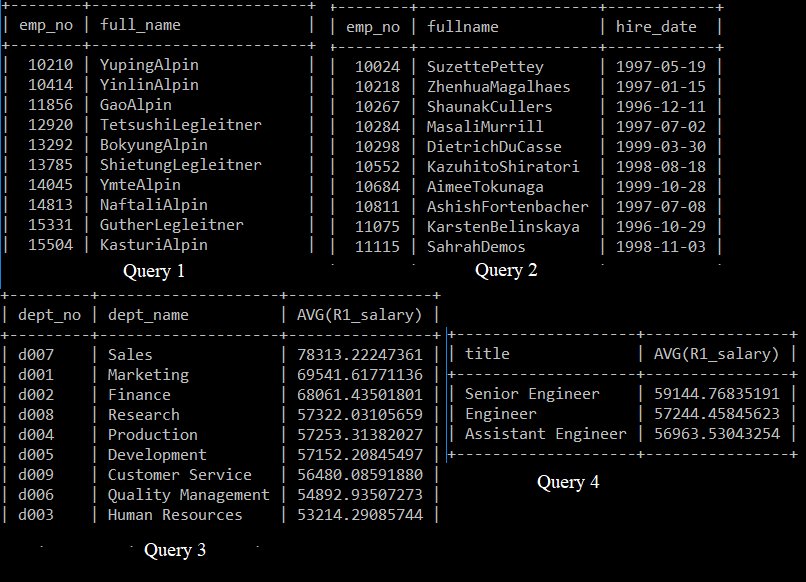
\includegraphics[scale = 0.65]{result.PNG}
\caption{Results}
\end{figure}
\end{document}
